\documentclass[a4paper]{jpconf}

\usepackage{graphicx} % for including graphics
\usepackage{amsmath} % useful maths macros, including \text
\usepackage{listings}
\usepackage{gensymb}
\usepackage{textcomp}
\usepackage{afterpage}
% \usepackage{apacite}
\usepackage{acronym}
% \usepackage{caption}
% \usepackage{subcaption}
\usepackage{tikz}
\usepackage{amssymb}
\usepackage{amsmath}
\usepackage{graphicx}
\usepackage{dcolumn}
\usepackage{hyperref} % tab this to get rid of colored hyper ref
\usepackage{color,units}
\usepackage{lineno}
\usepackage{xspace}
\usepackage{mathtools}
\usepackage{physics}
\usepackage{acronym}
\usepackage{subfigure}
\usepackage{multirow}
\usepackage{tikz}
% \usepackage{booktabs}
\usepackage[bibstyle=ieee,citestyle=numeric-comp]{biblatex} % the cite style lets multiple refs in one bracket
\addbibresource{refs.bib}
\renewcommand*{\multicitedelim}{\addcomma} 



% \newcommand{\texttt{Bilby}}{\texttt{Bilby}~}
% \newcommand{\texttt{emcee}}{\texttt{emcee}~}
% \newcommand{\texttt{ptemcee}}{\texttt{ptemcee}~}
% \newcommand{\texttt{Nessai}}{\texttt{Nessai}~}
% \newcommand{\texttt{VItamin}}{\texttt{VItamin}~}
% \newcommand{\texttt{Bilby}pipe}{{\sc bilby\_pipe}\xspace}
% \newcommand{\lalinference}{\texttt{LALInference}~}
% \newcommand{\texttt{dynesty}}{\texttt{dynesty}~}
% \newcommand{\texttt{cpnest}}{\texttt{cpnest}~}
% \newcommand{\nflows}{\texttt{nflows}~}
% \newcommand{\pytorch}{{\sc PyTorch}\xspace}
% \newcommand{\corner}{{\sc corner}\xspace}
% \newcommand{\matplotlib}{{\sc matplotlib}\xspace}
% \newcommand{\seaborn}{{\sc seaborn}\xspace}
% \newcommand{\numpy}{{\sc NumPy}\xspace}
% \newcommand{\scipy}{{\sc SciPy}\xspace}
% \newcommand{\pandas}{{\sc pandas}\xspace}
% \newcommand{\python}{{\sc Python}\xspace}
\newcommand{\imrphenomp}{\texttt{IMRPhenomPv2}}
\newcommand{\pycbc}{\texttt{PyCBC}}

% \raggedbottom % just incase it doesnt work nicely...
% \setlength{\parskip}{0pt}

\newcommand{\RNum}[1]{\uppercase\expandafter{\romannumeral #1\relax}}

% \newcommand{\figwidth}{8.6cm}
% \newcommand{\onehalffigwidth}{12.9cm}
% \newcommand{\doublefigwidth}{17.2cm}
% \newcommand{\montefigwidth}{11cm}
\newcommand*{\checktikz}[1][]{\tikz[x=1em, y=1em]\fill[#1] (0,.35) -- (.25,0) -- (1,.7) -- (.25,.15) -- cycle;}


\setlength{\footskip}{20pt}

\begin{document}
\title{Versatile deep-learning: Monte Carlo methods for gravitational wave inference}

\author{Project No: 628}

\address{\textit{SUPA, School of Physics and Astronomy\\University of Glasgow\\Glasgow G12 8QQ, United Kingdom}}


\begin{abstract}
In the era of multi-messenger astronomy, deep-learning approaches to parameter estimation are gaining significant traction in an effort to speed up sky localisation for rapid electromagnetic follow-up. Of these approaches, many implement variational inference techniques to obtain drastic speed increases over traditional methods. Variational inference compromises on versatility in pursuit of speed by avoiding likelihood calculations. However, these likelihoods are key to many diagnostic frameworks and so the technique remains significantly inflexible in their absence. In this paper, we present a novel method of estimating these likelihoods using Monte Carlo approximations to increase the versatility of our variational inference model. We start by presenting our established \texttt{VItamin} model’s capabilities of increasing parameter estimation sampling rate by more than 6 orders of magnitude compared to traditional methods. We then go on to present the results of our likelihood estimates and show that they are qualitatively self-consistent, followed by deriving an error relation to compare tolerances with other sampling algorithms. We finally present an application of this increased versatility by using an importance sampling framework to reweight our \texttt{VItamin} results relative to a \texttt{dynesty} target to improve our initial results by a process called likelihood reweighting. 
\end{abstract}

\acrodef{GW}[GW]{gravitational wave}
\acrodef{BBH}[BBH]{binary black hole}
\acrodef{EM}[EM]{electromagnetic}
\acrodef{CBC}[CBC]{compact binary coalescence}
\acrodef{BNS}[BNS]{binary neutron star}
\acrodef{NSBH}[NSBH]{neutron star black hole}
\acrodef{PSD}[PSD]{power spectral density}
\acrodef{ELBO}[ELBO]{evidence lower bound}
\acrodef{LIGO}[LIGO]{advanced Laser Interferometer Gravitational wave Observatory}
\acrodef{CVAE}[CVAE]{conditional variational autoencoder}
\acrodef{VAE}[VAE]{variational autoencoder}
\acrodef{KL}[KL]{Kullback--Leibler}
\acrodef{GPU}[GPU]{graphics processing unit}
\acrodef{LVC}[LVC]{LIGO-Virgo Collaboration}
\acrodef{PP}[p-p]{probability-probability}
\acrodef{SNR}[SNR]{signal-to-noise ratio}
\acrodef{DL}[DL]{deep-learning}
\acrodef{PE}[PE]{parameter estimation}
\acrodef{SIR}[SIR]{sampling-importance resampling}
\acrodef{VI}[VI]{variational inference}
\acrodef{NS}[NS]{nested sampling}
\acrodef{MCMC}[MCMC]{Markov Chain Monte Carlo}
% \acrodef{tf1}{tf1}{tensorflow}
%%%%%%%%%%%%%%%%%%%%%%%%%%%%%%%%%%%%%%%% INTRO %%%%%%%%%%%%%%%%%%%%%%%%%%%
\section{Introduction}\label{intro}

From the first hypothesis of gravitational waves in 1916~\cite{einstein1}, to the first direct detection of a binary black hole merger by the \ac{LIGO}~\cite{advancedLIGO} in 2015~\cite{abbott2016observation}, we continually find ourselves at the forefront of discovery when studying gravitational physics. As theorised in general relativity (GR), rotating massive objects release gravitational radiation in the form of gravitational waves, which cause ripples and deformations in the fabric of space-time. Signals from these massive objects can be divided into two general categories, continuous gravitational wave (CW) signals and transient gravitational wave (GW) signals. There is currently a high volume of work concerning CWs~\cite{bayley2019soap} and even significant effort to implement \ac{DL} techniques for imrproved detection~\cite{bayley2020soapML,cwml2019}. However in this paper, we solely focus on GWs, in particular GWs arising from compact binary coalescences (CBCs). CBCs describe the violent coalescence of stellar-mass black holes and neutron stars in 3 stages of inspiral, merger and ringdown. As these stellar-mass binaries merge, they expel an incredible amount of gravitational radiation, resulting in GW signatures at a frequency-range that is detectable by a network of ground-based detectors on Earth~\cite{advancedVIRGO,kagra,UNNIKRISHNAN_2013}. Detectors are highly-sensitive square-kilometre laser interferometers that can detect these GW signals from their imprint on detector strain from space-time deformations. The exact morphology of the GW signal can be reconstructed from the incident strain pattern in the form of a GW waveform. Template waveforms are modelled using computational numerical relativity~\cite{PhysRevLett.95.121101} and effective one-body formalisms~\cite{PhysRevD.59.084006} to solve GR equations. Creating high-quality template waveform banks and noise realisations are key to GW detection as LIGO software uses these template banks with additive noise injections to simulate real GW signals for matched filtering~\cite{PhysRevD.60.022002} analysis through specific \texttt{PyCBC}~\cite{pycbc2016} and \texttt{GstLal}~\cite{gstlal_gen1_2017,gstlal_gen2_2019} detection pipelines. Having released data for their first two and a half observing runs (O1,O2,O3a)~\cite{BBHo1,gwtc1,gwtc2} and with the O3b data-release expected later this year, an increasing number of detected events promise to keep LIGO research at the forefront of new science.

%%%%%%%%%%%%%%%%%%%%%%%%%%%%%%%%%%%%%%%% INTRO: PE %%%%%%%%%%%%%%%%%%%%%%%%%%%

\subsection{Parameter Estimation}\label{intro:pe}

\begin{table}[t]
	\centering
	\caption{The full \ac{PE} parameter range presented alongside the subset of inferred parameters highlighted with prior boundary values.}
	\begin{tabular}[t]{lcccc}
		\br
		parameter name & symbol & status & value & units\\
		\hline
		mass 1 & $m_1$ & inferred  & 35-80 & \(\textup{M}_\odot\)\\
		mass 2 & $m_2$ & inferred & 35-80 & \(\textup{M}_\odot\)\\
		luminosity distance & $d_{\text{L}}$ & inferred & 1-3 & Gpc\\
		time of coalescence & $t_{0}$ & inferred & 0.65-0.85 & s\\
		inclination & $\Theta_{jn}$ & inferred & 0-$\pi$ & rad\\
		polarisation & $\psi$ & inferred & 0-$\pi$ & rad\\
		\hline
		right ascension & $\alpha$ & fixed & 0 & rad\\
		declination & $\delta$ & fixed & 0 & rad\\
		spins (x6) & - & fixed & 0 & -\\
		\hline
		phase at coalescence & $\phi_{0}$ & marginalised & 0-$2\pi$ & rad\\
		\br
	\end{tabular}
	\label{tab:params}
\end{table}

Once LIGO has detected a GW signal, the next task is to infer the parameters of the merger through a technique called parameter estimation (PE). CBCs are typically described by 15 parameters, as detailed in Table 1, with 8 intrinsic parameters for masses and spins and 7 extrinsic parameters to describe the location and orientation of the merger relative to the detector. In a similar framework to detection, these parameters can be inferred from their waveform signature, modelled against a bank of template waveforms. The optimum way to approach this inverse-problem is shown in~\cite{2009CQGra..26o5017S} to be Bayesian inference, a technique built upon the mathematical framework of Bayesian statistics~\cite{bayesog}. This statistical framework differs from classical statistics by approaching probability as a degree of belief relative to a combination of current data and prior knowledge, instead of current data in isolation. Bayesian statistics is based on Bayes’ Theorem~\cite{Bayestheorem} which, applied to our inference problem, can be represented as

\begin{align}\label{eq:bayes_exact} 
	p(x|y) = \frac{{\cal L}(y|x) p(x)}{\cal Z} ,
\end{align}

where $x$ represents the inference parameters, $y$ is the noisy GW waveform, $p(x|y)$ is the posterior probability, read as `the probability of the parameters given the input data’, ${\cal L}(y|x)$ is the likelihood, $p(x)$ is the prior knowledge of the parameters and ${\cal Z}$ is the Bayesian evidence. The Bayesian evidence can be evaluated from the likelihood and prior by

\begin{align}\label{eq:bayes_evidence} 
{\cal Z} = \int dx {\cal L}(y|x) p(x),
\end{align}

where ${\cal Z}$ is a very useful measurement to quantify the results of a Bayesian inference run~\cite{sivia2006textbook}. However, in the framework of PE we are only interested in the shape of the posterior so ${\cal Z}$ becomes a normalisation constant which can be ignored. This means we can represent Bayes’ Theorem with respect to GW PE as 

\begin{align}\label{eq:bayes_prop} 
	p(x|y) &\propto {\cal L}(y|x) p(x). 
\end{align}

\begin{table}[t]
	\centering
	\caption{Required run-times for traditional and \ac{DL} sampling methods to produce benchmark $\mathcal{O}(10000)$ posterior samples. Run-times quoted for \ac{DL} algorithms do not include training time.}
	\begin{tabular}[t]{l|lcc} 
				\br
				sampler & algorithm & deep-learning & run-time (s)\\
				\hline
				\texttt{emcee}~\cite{emcee} & MCMC~\cite{mcmc_og} & X  &  32070\\
				\texttt{ptemcee}~\cite{ptemcee} & MCMC & X & 24372\\
				\hline
				\texttt{dynesty}~\cite{dynesty} & NS~\cite{skilling2006} & X & 19400\\
				\texttt{cpnest}~\cite{cpnest} & NS & X &  26202 \\
				\texttt{Nessai}~\cite{williams2021nested} & NS & \checktikz & 9372\\
				\hline
				flows~\cite{stephengreen2020} & VI~\cite{1904.06264} & \checktikz & 2\\
				\texttt{VItamin}~\cite{vitpaper} & VI & \checktikz & $1\times 10^{-1}$\\
				\br
	\end{tabular}
	\label{tab:speed}
\end{table}

As the posterior describes the parameter space, the dimension of the posterior distribution matches the number of inferred parameters, and so, evaluation of this high-dimensional probability becomes infeasible analytically. Instead of trying to evaluate the probability surface, we stochastically sample from it to create an informed estimate of the posterior distribution. The main software used for LIGO PE is \texttt{Bilby}~\cite{bilby} and \texttt{LALInference}~\cite{lalinference} which contain a selection of samplers operating on a \ac{MCMC}~\cite{emcee,ptemcee} or \ac{NS} algorithm~\cite{dynesty,cpnest}. NS~\cite{Skilling2004} and MCMC~\cite{Metropolis1953,Hastings1970,Hogg} algorithms work by stochastically sampling from the prior distribution and assigning it a likelihood value by comparing the input data to a template waveform generated from the prior sample. Both methods then accept or reject this likelihood value according to their individual algorithmic methodology until the optimum posterior is estimated. An added benefit of NS samplers is their versatile ability to evaluate the Bayesian evidence for a sample run. These traditional sampling methods provide high quality posterior estimates but are very time-consuming due to repeated likelihood evaluates. The significant computational cost of these likelihood evaluations is demonstrated in Table~\ref{tab:speed}, with NS and MCMC sampling run-times $\mathcal{O}(10)$ hours. Due to this time-consuming nature, much recent work has been focused on high-performance and high-throughput computing techniques to reduce this run-time and increase sampling speed by $\mathcal{O}(1\textup{-}2)$ orders of magnitude~\cite{smith,purrer,gpu_inference,gpu_rit,2016PhRvD..94d4031S,2019PhRvD..99h4026W,2019PhRvD.100d3030T}. 

In the first LIGO observing run, there was a focus on accurate PE to enable new tests of relativistic astrophysical theories~\cite{GW170817_Hubble,GW150914_gr,Schutz}. However, detecting the first binary neutron star CBC (GW170817)~\cite{GW170817_properties} in the second observing run, birthed a new field of multi-messenger astronomy~\cite{GW170817_mma}, which requires fast PE for rapid sky localisation for follow-up observations of electromagnetic counterparts. This shift towards new science motivates the inception of new PE methods that allow for sub-second sampling. An ideal solution to this run-time bottleneck is the implementation of \ac{DL} methods. There is a high volume of current work on implementing DL techniques into both the detection and PE pipelines~\cite{PhysRevLett.120.141103}. A recent review~\cite{mlreview2020} discusses the potential for DL implementations to transform every aspect of CBC detection, and places even further emphasis on the motivation for rapid PE. Concerning \ac{DL} approaches, some works have been focused on enhancing traditional sampling methods~\cite{williams2021nested} by reducing the effective number of likelihood calculations during inference. Other implementations~\cite{stephengreen2020,vitpaper} look to completely replace traditional methods, circumventing the need for likelihood evaluations completely, using a technique called \ac{VI}~\cite{1904.06264}. Once trained, these models boast sub-second run-times, as seen in Table 2.

%%%%%%%%%%%%%%%%%%%%%%%%%%%%%%%%%%%%%%%% INTRO:DL %%%%%%%%%%%%%%%%%%%%%%%%%%%
\subsection{Deep-learning Approaches}\label{intro:dl}

DL is a specific branch of machine learning that uses deep neural networks (DNNs). The many layers of DL algorithms make them very efficient in deciphering relevant features of raw data in an unsupervised framework, as is required for GW inference. A specific class of DL algorithms that have proven to be very useful for GW PE are deep generative models. Deep generative modelling is a technique that trains DNNs to model distributions found in training data, making it particularly useful for approximate inference~\cite{1807.03653}. The rapid progress of applied deep generative modelling research has split the field into many different specialised architectures, each with individual strengths and weaknesses. A recent review~\cite{bond2021deep} acknowledges this fragmentation of the research field and looks to provide a standard framework of its current status. To do this, they present direct comparisons between architectures for important aspects in the VI pipeline, such as training speed and sample quality. Looking at these comparisons, two architectures stood out to be particularly well-suited for our specific GW PE use case. 

The first architecture, normalising flows, have been well-studied as a successful GW inference candidate~\cite{williams2021nested,papamakarios2019normalizing}. Normalising flows work by mapping the input distribution to an auxiliary normal distribution, using an invertible linear transform. This change of basis allows easy sampling at high dimensions, due to the simple structure of the auxiliary distribution. However, the restrictions on the transform to be linear and invertible, as well as the high-dimensional auxiliary distribution, make normalising flows hard to train for the parameter spaces required for PE. For this reason, we have opted to use the second architecture recommended for use in GW inference, conditional variational autoencoders (CVAEs). CVAEs are comprised of two DNNs, the first encodes the input distribution into a lower dimensional latent space distribution, whilst the second decodes this latent representation to reconstruct the original data. The conditional aspect of the architecture comes from the input of data labels in the training phase, extending to a semi-supervised framework. We present our CVAE, designed particularly for VI of GW waveforms, aptly name \texttt{VItamin}. We follow on from the peer-reviewed \texttt{VItamin} paper~\cite{vitpaper} henceforth, paper 1.

%%%%%%%%%%%%%%%%%%%%%%%%%%%%%%%%%%%%%%%% INTRO:VIT %%%%%%%%%%%%%%%%%%%%%%%%%%%
\subsection{\textup{\texttt{VItamin}}: User-friendly Inference}\label{intro:vit}

\begin{figure}
	\centering
	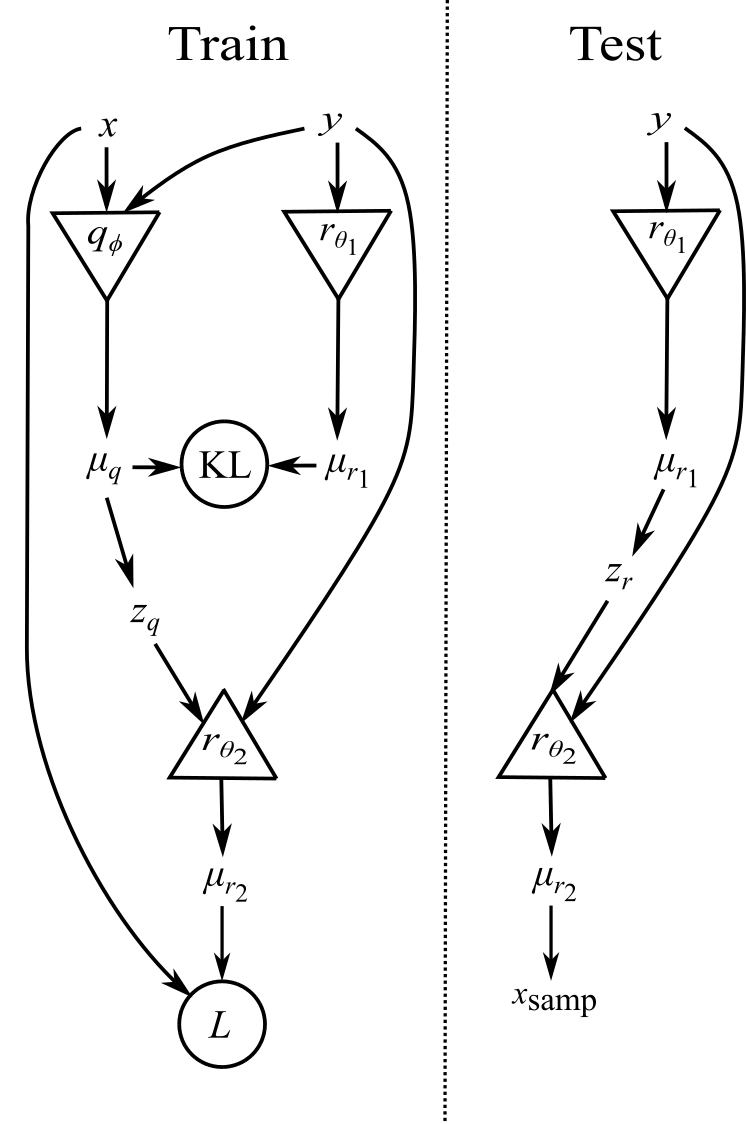
\includegraphics[width=.5\linewidth]{figs/network_setup.png}
	\caption{The structure of \texttt{VItamin} \ac{CVAE} network. \textbf{Left:} Training procedure to minimise total cost function ($H$) from its constituent cost functions, KL-divergence (KL) and reconstruction loss ($L$) using Eq.~\ref{eq:cost_approx}. Noisy GW data ($y$) and true parameter values ($x$) are incident on recognition network ($q_\phi$) whilst only $y$ is incident on encoder network ($r_{\theta_1}$). These two networks produce latent distributions ($\mu_{q,r_1}$), a sample ($z_q$) is drawn from the encoder latent distribution to construct decoder network ($r_{\theta_2}$) with corresponding distribution ($\mu_{r_2}$) trained to reconstruct the true posterior $p(x|y)$. \textbf{Right:} \texttt{VItamin} structure in production, conditional only on $y$. A sample ($z_r$) is drawn from the encoder network latent distribution and the decoder network outputs proposal posterior samples ($x_\textup{samp}$). Figure reproduced from paper 1~\cite{vitpaper}.}
	\label{fig:vit_flow}
\end{figure}

Presented in paper 1, \texttt{VItamin} is a \ac{CVAE} that is conditioned on input noisy GW waveform data ($y$), which seeks to generate a proposal posterior $r_\theta(x|y)$ to reconstruct the true posterior $p(x|y)$ seen during training. The constituent DNNs are trained by minimising a cross-entropy cost function

\begin{align}\label{eq:cross_ent} 
H(p,r_\theta) &= -\int dx\, p(x|y) \log r_{\theta}(x|y),
\end{align}

which is inherently minimised when the proposal posterior tends to the true posterior. The proposal posterior is parameterised on the output of the encoder $r_{\theta_1}(z|y)$ and decoder $r_{\theta_2}(x|y,z)$ networks as follows

\begin{align}\label{eq:prop_post}
r_{\theta}(x|y) = \int dz\,r_{\theta_1}(z|y)r_{\theta_2}(x|y,z).
\end{align}

Here, the $\theta$ subscripts represent tunable training parameters and $z$ represents samples drawn from the lower dimensional latent space distribution. Starting from its continuous form (Eq.~\ref{eq:cross_ent}), we can derive an approximate bound for the cross-entropy, parameterised further on a recognition network $q_{\phi}(z|x,y)$, based on an independet set of tunable parameters $\phi$. The derivation (detailed in paper 1) uses a stochastic integral approximation to allow the cost function to be iterable over a training batch $N_b$. The final form of the cross-entropy cost function is given by the bound

\begin{align}\label{eq:cost_approx} H \lesssim
\frac{1}{N_b}\sum_{n=1}^{N_{\text{b}}}&\Big[\overbrace{-\log
	r_{\theta_{2}}(x_{n}|z_{n},y_{n})}^{L}+\overbrace{\text{KL}\left[q_{\phi}(z|x_{n},y_{n})||r_{\theta_{1}}(z|y_{n})\right]}^{\text{KL}}\Big],
\end{align}

which is also represented graphically in Fig.~\ref{fig:vit_flow}. The total cost function is constructed as a basic sum of 2 constituent cost functions. The Kullback–Leibler (KL)-divergence quantifies the convergence of $r_{\theta_1}$ and $q_{\phi}$ latent space distributions, minimised when both distributions are equal. The reconstruction cost $L$ measures how well $r_{\theta_2}$ predicts the true parameters $x$. Concerning notation throughout this paper, inside the remit of model training and validation, $p(x|y)$ represents the true posterior formed from the training data $x$ parameters. However, later when we start to compare with other algorithms, $p(x|y)$ represents the target posterior created using the \texttt{dynesty} sampling algorithm. Further details on our specific training procedure are presented in Section~\ref{methods:training}. 

From Table~\ref{tab:speed}, we can see the speed increase of \texttt{VItamin} compared to the traditional sampling methods and other DL frameworks. However, a consequence of this speed is limited network versatility. In this paper, we present a method to estimate the likelihoods of \texttt{VItamin} proposal posterior samples, using Monte Carlo approximations to increase the versatility of \texttt{VItamin}. This would align \texttt{VItamin} with the abilities of NS algorithms, with the end goal of estimating the Bayesian evidence, using Eq.~\ref{eq:bayes_evidence}. A particularly useful consequence of obtaining likelihood evaluations, is the ability to resample the proposal posterior using a technique called likelihood reweighting. A recent paper~\cite{resample_aus} showed this method to be successful in improving their approximate posterior results. In their paper, they used an approximate waveform generator~\cite{IMRPhenomD} to construct a proposal posterior using the \texttt{Bilby} implementation of \texttt{cpnest}. They then reweighted these proposal samples according to their likelihood ratio with a more complete, but computationally expensive target waveform generator~\cite{NRHybSur3dq8}, using a process called \ac{SIR}~\cite{brian2006resampling}. They found that, through likelihood reweighting, they could effectively simulate drawing samples from the target posterior without ever having to run the sampling algorithm on the computationally expensive waveforms. Once we have estimated our proposal likelihoods, we look to use a similar \ac{SIR} approach to improve the results of \texttt{VItamin} by reweighting our samples according to their likelihood ratio with the target posterior. We choose to use the \texttt{Bilby} implementation of \texttt{dynesty} for our target posterior due to its improved sampling speed over \texttt{cpnest}, as shown in Table~\ref{tab:speed}.

The structure of the paper is as follows. In Section~\ref{method}, we set out the framework for training our \texttt{VItamin} model on a reduced parameter space and describe the Monte Carlo methods used for likelihood evaluations and reweighting. In Section~\ref{results}, we discuss the quality of these proposal likelihoods using qualitative self-consistency and quantitative reproducibility tests. We then go on to evaluate the suitability of the \ac{SIR} method for our resampling test case, compared to the success of \cite{resample_aus}. In Section~\ref{conc}, we contextualise our results in the wider field of rapid PE, by reiterating the significance of adding versatility to our \texttt{VItamin} model. We then finally set out a road map of related future work.

\begin{figure}
	\centering
	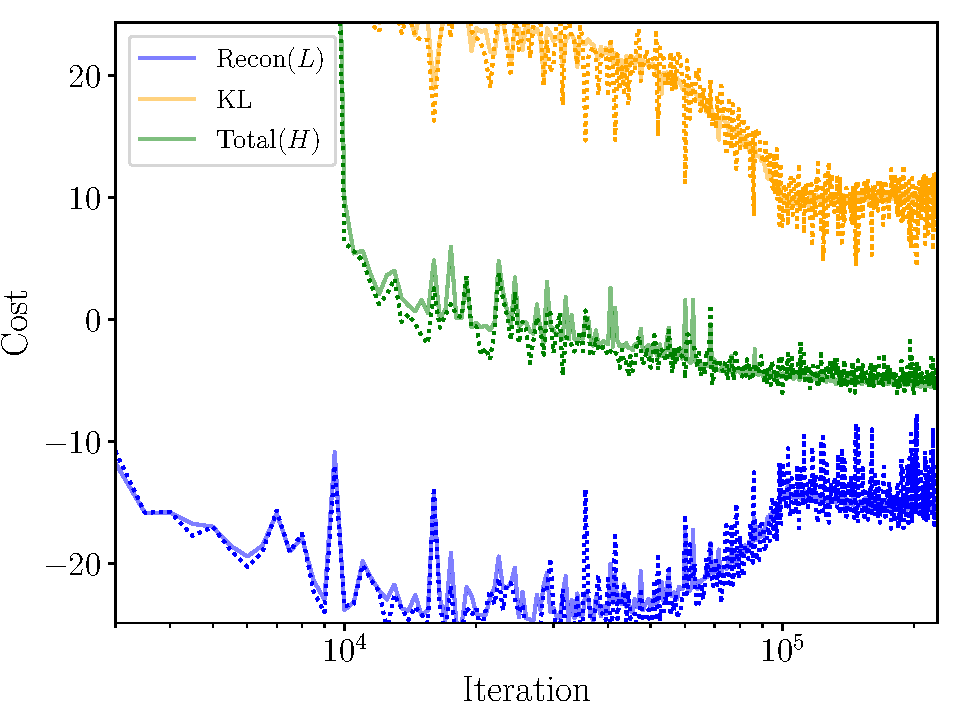
\includegraphics[width=.5\linewidth]{figs/cost.pdf}
	\caption{Cost as a function of training batch iteration. We show total cost (green) and its constituent functions KL-divergence (yellow) and reconstruction loss (blue), where total cost function is a simple sum of both constituents (Eq.~\ref{eq:cost_approx}). Solid lines correspond to training data cost and dotted lines represent validation cost. The convergence of training and validation cost indicates a lack of overfitting. The progress of this model was deliberately stopped prematurely as indicated by the total cost gradient never levelling off. }
	\label{fig:cost}
\end{figure}

% %%%%%%%%%%%%%%%%%%%%%%%%%%%%%%%%%%%%%%%% METHODS %%%%%%%%%%%%%%%%%%%%%%%%%%%
\section{Methodology}\label{method}

\subsection{Model Training}\label{methods:training}

Our \texttt{VItamin} network was constructed as in Fig.~\ref{fig:vit_flow}, with the base network hyperparameters detailed in Table~\RNum{3} of paper 1. Small modifications were made to this base structure, namely a reduction in latent space dimension to account for our lower dimensional sub-parameter space. We chose to infer a subset of 6 parameters in this test case (see Table~\ref{tab:params}) for two reasons. The first was to save time generating our target posterior using \texttt{dynesty}, the 10000 target samples were generated in $\mathcal{O}(3)$ hours compared to the benchmark 6 hours quoted in Table~\ref{tab:speed}. The second was the strict requirement on all inferred parameters to be defined on uniform priors for likelihood calculations, as detailed in Section~\ref{method:monte}. Due to the sinusoidal prior on declination, we were unable to infer sky parameters so we decided on a single-detector PE run in the absence of sky-localisation capabilities. We then trained the model by minimising $H$ in its iterable approximate form (Eq.~\ref{eq:cost_approx}). Figure~\ref{fig:cost} shows the progress of \texttt{VItamin} training with $H$ decreasing with training iteration. The behaviour seen between $10^4$ and $10^5$ iterations is a consequence of ramping $L$ up to find the optimum gradient descent for $H$.

To quantify the progress of model training, it is useful to set aside some labelled data that the model does not see in the training batch called a validation set. This tests to see if the model is really improving with training iteration or has simply memorised the training data, giving a misnomer $H$ decrease. This memorising of training data is called overfitting and occurs when the wrong configuration of training parameters is used. Most tunable training parameters, such batch size and number of epochs were kept consistent with paper 1 and the dotted lines on Fig.~\ref{fig:cost} show validation cost aligns with training cost, indicating there is no overfitting and the model is successfully training. The number of training iterations was initially set to $10^6$, however training was stopped early to ensure the proposal posterior from \texttt{VItamin} $r_\theta(x|y)$ was sufficiently different from the \texttt{dynesty} target posterior $p(x|y)$ to allow resampling improvements to be more visible on plots, see Section~\ref{results:resample}. The fact that the $H$ curve does not flatten in Fig.~\ref{fig:cost} indicates our model is not fully trained. 

\begin{figure}
	\subfigure{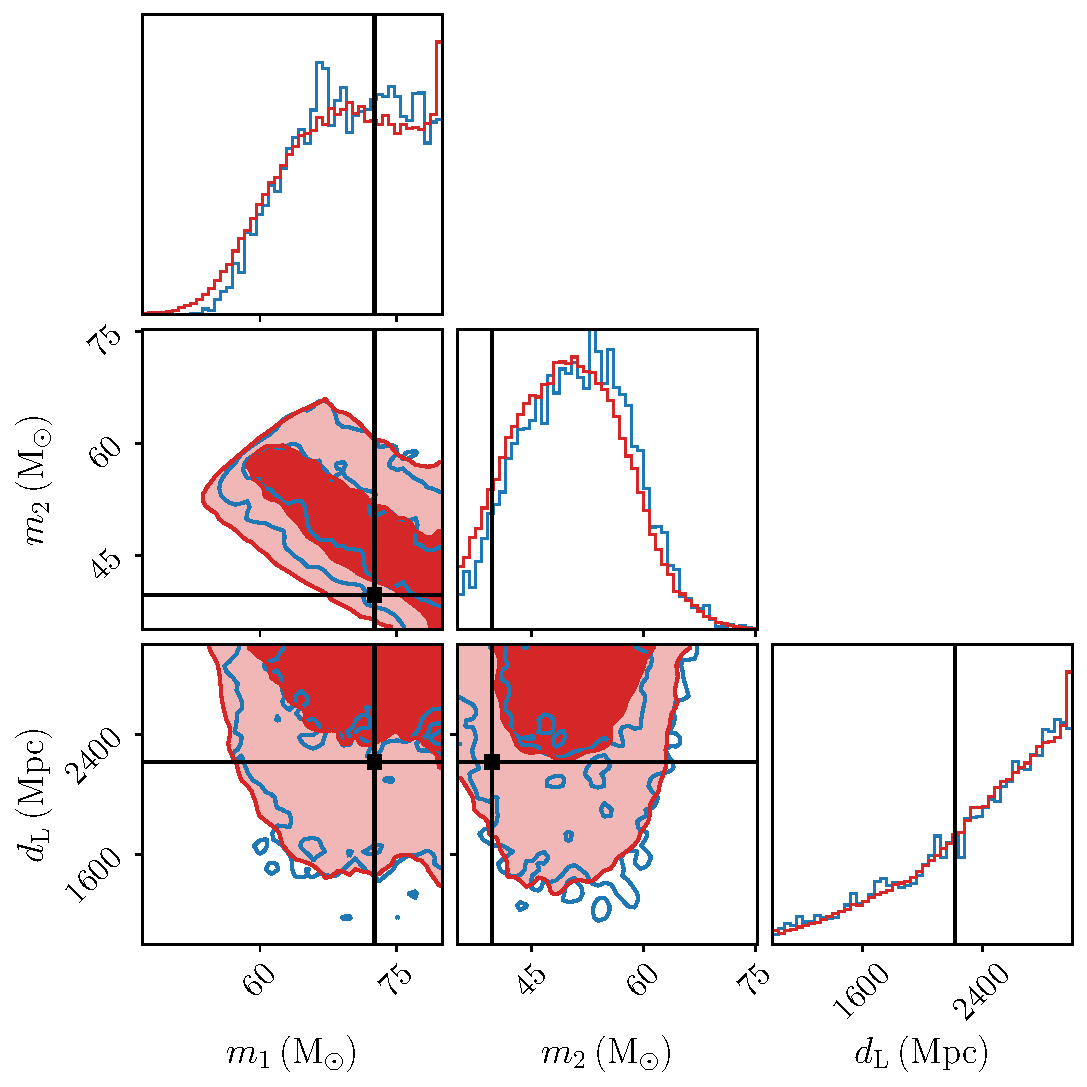
\includegraphics[width=.5\linewidth]{figs/vit_train_corner1.pdf}}
	\subfigure{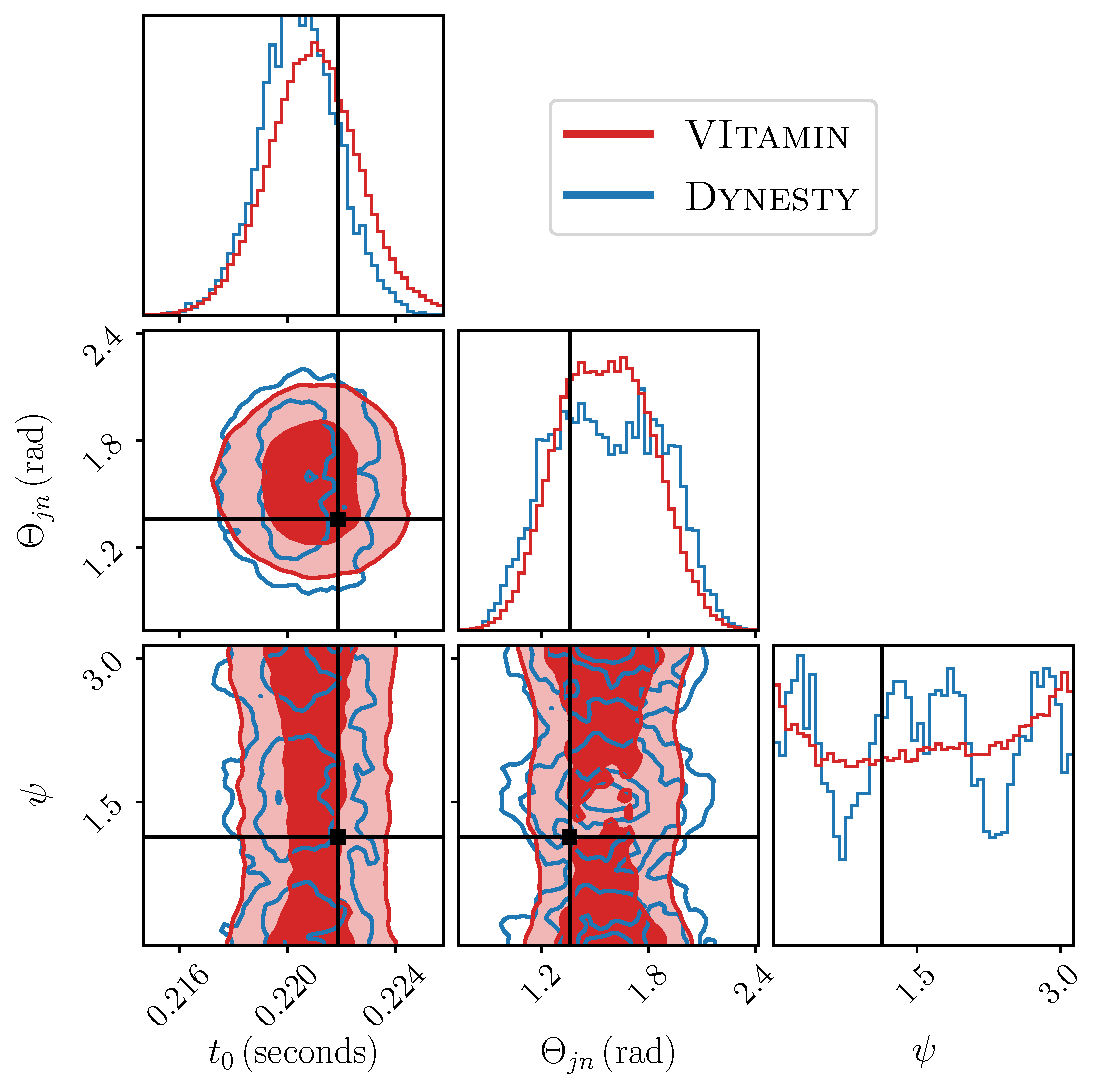
\includegraphics[width=.5\linewidth]{figs/vit_train_corner2.pdf}}
	\caption{Partial corner plot for proposal and target posterior distributions. We show our 100000 \texttt{VItamin} proposal posterior (red) overlaid with our 10000 \texttt{dynesty} target  posterior (blue) for the 6 inferred parameters identified in Table~\ref{tab:params}. True $x$ parameters are shown in black with the 2D contours representing the 50\% and 90\% credible interval of the posteriors. Order of magnitude sample discrepancy accounts for increased smoothness of \texttt{VItamin} posterior with both overlapping for the uni-modal distributions. For the inclination and polarisation multi-modal target posterior, there exists regions of under-sampling from \texttt{VItamin}.}
	\label{fig:vit_train_corner}
\end{figure}

From this partially trained model, we generated 2 sets of \texttt{VItamin} samples. An initial set of 5000 was created, dictated by empirical findings that 5000 was the minimum number of samples required for smooth posterior plots. A second set of 100000 was then created to allow for sufficient resampling as detailed in Section~\ref{method:monte}. This set of 100000 proposal samples was compared to the 10000 target samples in Fig.~\ref{fig:vit_train_corner}. This partial corner plot shows the cross-section representation of the proposal and target posteriors, allowing meaningful visualisation of the complex multi-dimensional probability surfaces. Here, the black points represent the position of the true parameters from our noisy GW signal in parameter space, and the 2D contours represent the 50\% and 90\% credible intervals of the individual posteriors. The 100000 \texttt{VItamin} and 10000 \texttt{dynesty} samples are shown, with the order of magnitude discrepancy accounting for the increased smoothness of \texttt{VItamin} curves. For the uni-modal distributions, the proposal approximates the target well with significant convergence. For the multi-modal distributions of inclination and polarisation parameters, the proposal significantly diverges from target as a consequence of incomplete training. This creates regions of under-sampling in the 2D representations which we aim to rectify by resampling.

\subsection{Likelihood Estimates}\label{method:monte}

Monte Carlo methods provide a framework for estimating hard-to-compute expectation values of continuous functions by evaluating the convergence of stochastic samples drawn from these functions~\cite{brian2006resampling}. This stochastic integral evaluation was key to the derivation of the approximate cost function $H$ (Eq.~\ref{eq:cost_approx}) from its continuous form $H(p,r_\theta)$ (Eq.~\ref{eq:cross_ent}), as detailed in paper 1. In its parametric form (Eq.~\ref{eq:prop_post}), $r_\theta(x|y)$ is an integral that is very hard to solve analytically. By expressing it as an expectation value 

\begin{align}\label{eq:monte_approx}
	r_{\theta}(x|y) =\,\mathbb{E}_{r_{\theta_1}(z|y)}r_{\theta_2}(x|y,z),
\end{align}

we can implement a Monte Carlo approximation to estimate the proposal posterior at a single point in parameter space $x_i$

\begin{align}\label{eq:monte_approx2}
r_{\theta}(x_i|y)\approx\frac{1}{N}\sum^{N}_{j=1}\left.r_{\theta_{2,j}}(x_i|y,z_j)\right|_{z_j\sim r_{\theta_1}(z_j|y)},
\end{align}

where $x_i$ is a single output sample from our trained network. By iteratively drawing $z_j$ samples from $r_{\theta_1}(z_j|y)$ to construct $r_{\theta_{2,j}}(x|y,z_j)$ and evaluating these decoder networks at $x_i$ over a batch size $N$, we can directly estimate the proposal posterior for $x_i$. Due to our deliberate choice of parameters with uniform priors and, as \ac{PE} does not require normalisation (Eq.~\ref{eq:bayes_prop}), it is straight forward to show that this proposal posterior estimate can also be approached as a likelihood estimation

\begin{align}\label{eq:post_like}
r_{\theta}(x_i|y) \sim {\cal L}_{\theta}(y|x_i),
\end{align}

where ${\cal L}_\theta(y|x_i)$ is the proposal likelihood of a single vitamin sample $x_i$.

\begin{figure}
	\centering
	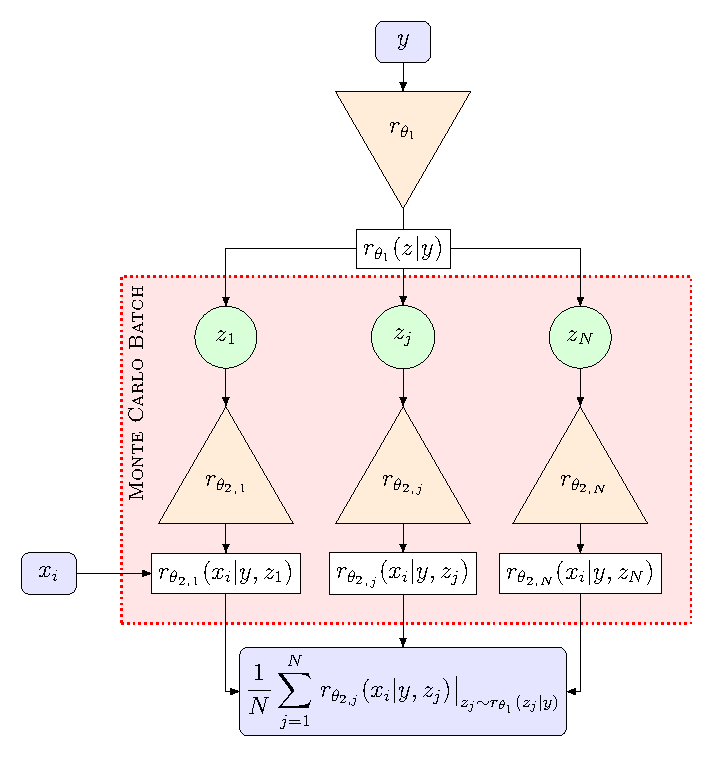
\includegraphics[width=.75\linewidth]{figs/tikz_monte.pdf}
	\caption{Flow diagram for estimation of proposal likelihood ${\cal L}_\theta(y|x_i)$ of a single proposal posterior sample ($x_i$) conditional on noisy GW data ($y$). Encoder network $r_{\theta_1}(z|y)$ is constructed as described in Section~\ref{intro:vit} and a batch of latent space samples ($z_{1:N}$) defined by Monte Carlo batch size $N$ are drawn to construct an array of parallel decoder networks $r_{\theta_{2,1:N}}(x|y,z_{1:N})$. Decoder networks are then evaluated in parallel at $x_i$ and combined using a Monte Carlo approximation (Eq.~\ref{eq:monte_approx2}) to output a single proposal likelihood estimate. $N$ is limited on hardware so can repeat Monte Carlo batch (red square) $R$ times in series to obtain an effective batch size $z_\textup{eff}=NR$.}
	\label{fig:monte_flow}
\end{figure}

A practical approach to this Monte Carlo approximation is shown in Fig.~\ref{fig:monte_flow}. A batch of $z_N$ samples are drawn from $r_{\theta_1}$ and ran through the \texttt{VItamin} network in parallel to reconstruct the likelihood of a single sample. We want $N$ to be as large as possible to outweigh the stochastic nature of Monte Carlo sampling, however this is limited by hardware. For reference, our \texttt{Nvidia Tesla V100} GPU allowed a maximum $N=65000$. A way to increase this further would be to run the Monte Carlo batch section (highlighted as a red box in Fig.~\ref{fig:monte_flow}) $R$ times in series to create an effective batch size $z_\textup{eff}=NR$. In practice, the $r_{\theta_2}$ networks are constructed using \texttt{tensorflow.v1}  (\texttt{tf.1})~\cite{tensorflow} and consist of separate complex distributions for the different constituent parameters of $x_i$, which need to be evaluated separately and combined later. To allow this combination to be a summation rather than a more costly product, the natural log of the proposal likelihood is evaluated as a proposal log-likelihood. 

Using these methods, we evaluate log-likelihoods for our set of 5000 and 100000 \texttt{VItamin} samples. However, as a consequence of our version of \texttt{VItamin} being written in discontinued \texttt{tf.1} at the time of work, there was a known memory leak issue in the code which limited our ability to maximise $z_\textup{eff}$. For the 5000 sample run, we were able to load the GPU with $N=65000$ and $R=4$ repetitions giving $z_\textup{eff}=260000$, however we were only able to run the 100000 samples with $z_\textup{eff}=25000$. The consequences of this order of magnitude discrepancy and further software limitations are dealt with in Section~\ref{results:repro}. For both sets of proposal samples, the target log-likelihoods were obtained using \texttt{Bilby}, ensuring the same noisy GW data and waveform generator was used as the initial \texttt{VItamin} proposal sample run.

\subsection{Likelihood Reweighting}\label{method:reweighting}

Importance sampling is a well-established method for drawing from a target distribution using only proposal samples and relative likelihoods~\cite{1592027}. \ac{SIR} is a Monte Carlo approximation of this technique which allows reweighting of the proposal distribution to add more importance to under-sampled regions compared to the target posterior, as discussed for the multi-modal distributions in Fig.~\ref{fig:vit_train_corner}. This is done by constructing a normalised weight function as a ratio of target and proposal likelihoods

\begin{align}\label{eq:weights}
w(y|x) \equiv \frac{{\cal L}(y|x)}{{\cal L}_{\theta}(y|x)}.
\end{align}

Following the methodology used in~\cite{resample_aus}, we start with the \ac{PE} version of Bayes’ Theorem for the target posterior (Eq.~\ref{eq:bayes_prop}), then multiply by unity with respect to the proposal likelihoods. Extracting the weight function from the right-hand side leaves only the proposal posterior

\begin{align}\label{eq:sir} 
p(x|y) &\propto \frac{{\cal L}_\theta(y|x)}{{\cal L}_\theta(y|x)}{\cal L}(y|x) p(x)\nonumber\\
&\propto w(y|x)\overbrace{{\cal L}_{\theta}(y|x) p(x)}^{r_{\theta}(x|y)},
\end{align}

which provides a way of drawing from the target posterior by weighted resampling of the proposal posterior. In~\cite{resample_aus}, a resampling function is derived to dictate the resampling ratio, that is, how many weighted samples to extract from the proposal posterior. However,~\cite{brian2006resampling} suggests a simpler benchmark resampling ratio of 20 gives sufficient results. As a proof-of-concept, we resample according to this simpler benchmark to extract 5000 weighted samples from our 100000 proposal samples.


% %%%%%%%%%%%%%%%%%%%%%%%%%%%%%%%%%%%%%%%% RESULTS %%%%%%%%%%%%%%%%%%%%%%%%%%%
\section{Results}\label{results}

\subsection{Self-consistency}\label{results:self_consist} %%%%%%%%%%%%%%

\begin{figure}
	\subfigure{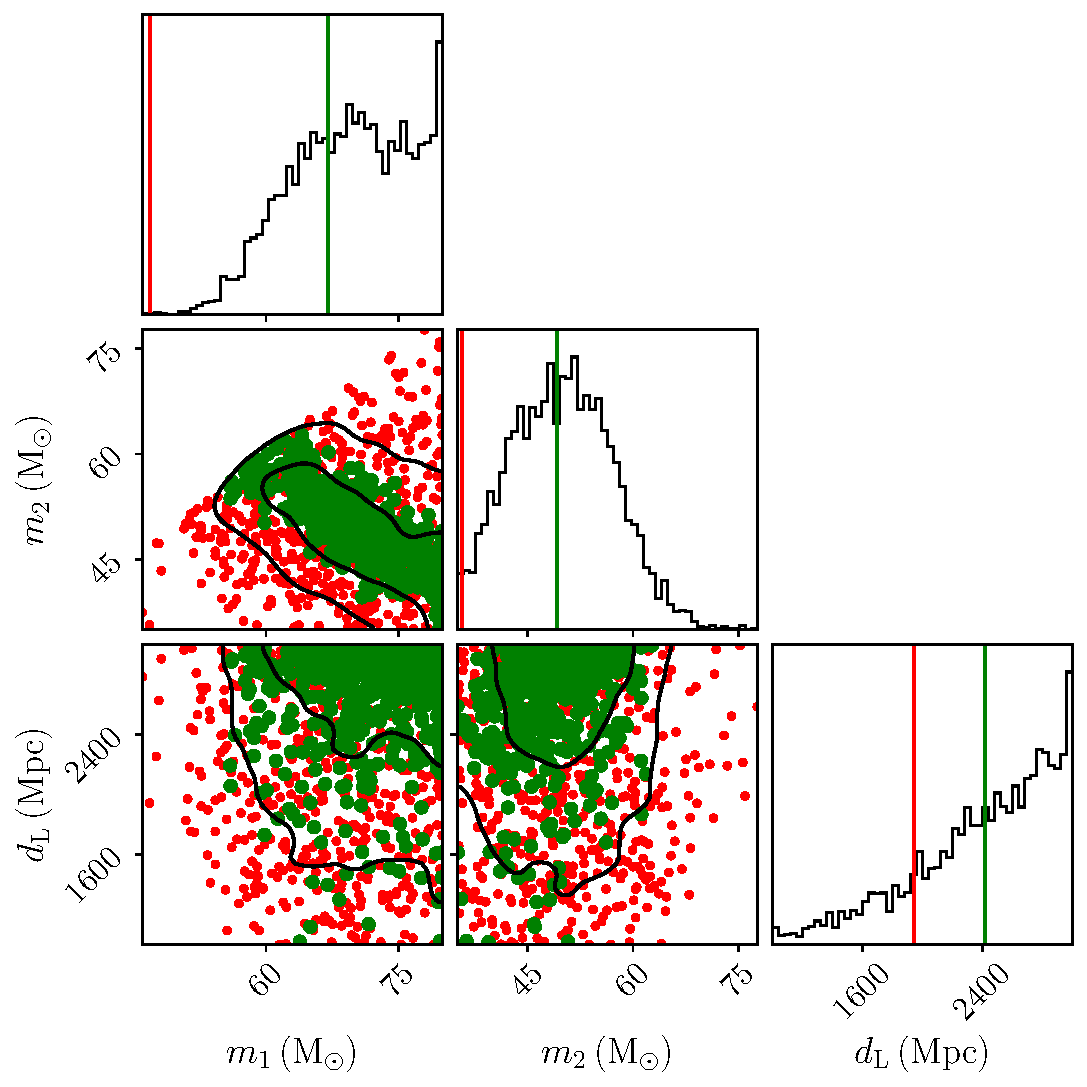
\includegraphics[width=.5\linewidth]{figs/self_consist1.pdf}}
	\subfigure{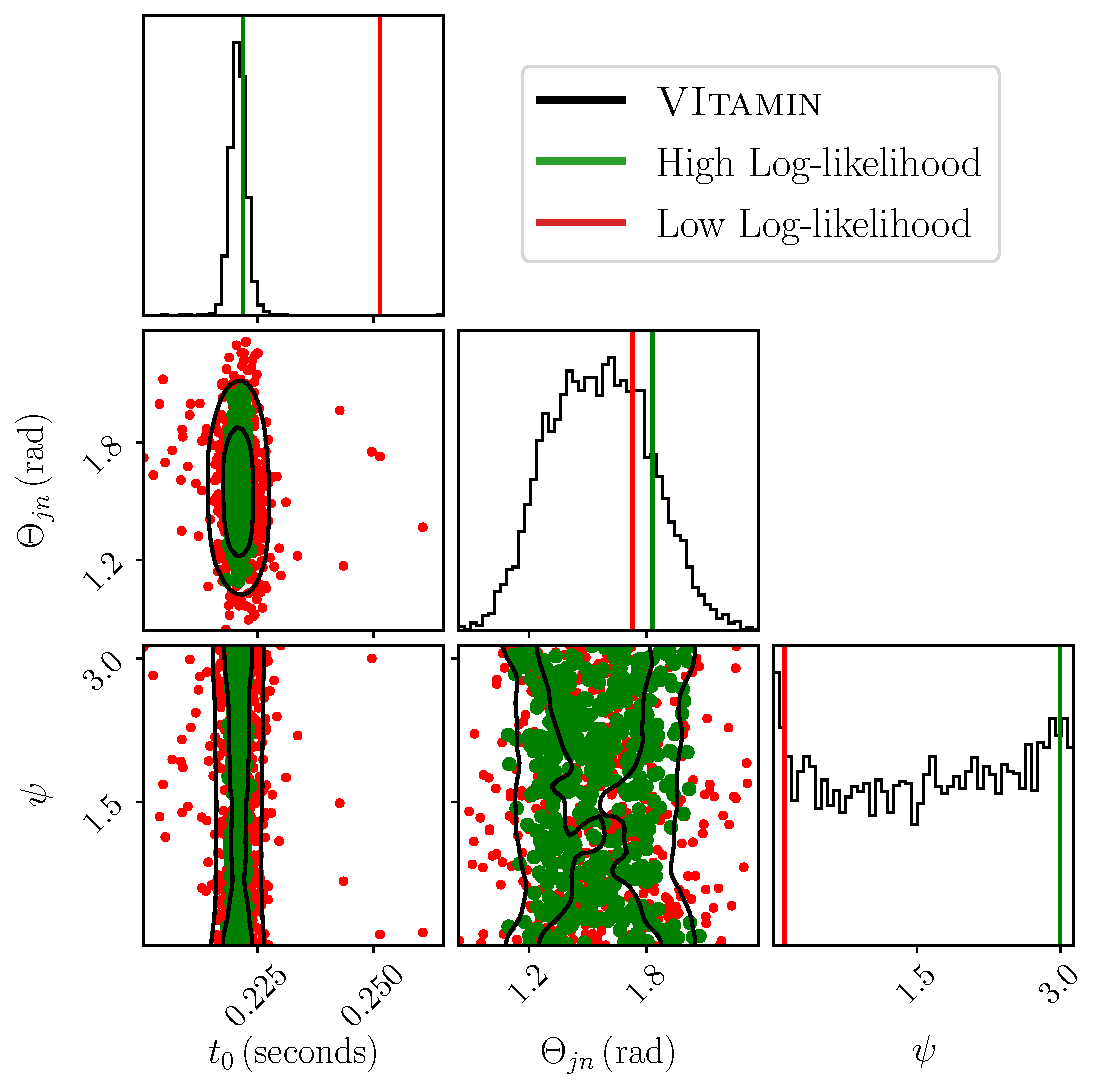
\includegraphics[width=.5\linewidth]{figs/self_consist2.pdf}}
	\caption{Partial corner plot of proposal posterior and log-likelihood estimates. We present our 5000 \texttt{VItamin} proposal posterior samples (black) with 2D contours representing the 50\% and 90\% confidence intervals. Samples with the highest 500 (green) and lowest 500 (red) log-likelihood estimates (calculated using Eq.~\ref{eq:monte_approx2}) are plotted over the 2D contours. For the 1D distributions, the single highest and lowest log-likelihoods are plotted. Self-consistency is seen explicitly in the uni-modal distributions, whereas the multi-modal distributions only exhibit clear self-consistency in the 2D plots.}
	\label{fig:self_consist}
\end{figure}

The first criterion of our proposal log-likelihoods is that they endure self-consistency. That is, higher log-likelihood values must correspond with samples in the centre of the proposal posterior and lower log-likelihood values must correspond with samples located in the tails of the distribution. This is an essential qualitative test to diagnose any internal methodological errors before comparing with target distributions. In Fig.~\ref{fig:self_consist}, we present another partial corner plot of our 5000 proposal posterior samples with the same 50\% and 90\% credible intervals in the 2D contours. We show the positions in parameter space corresponding to the highest 500 (green) and lowest 500 (red) proposal log-likelihood estimates. For the 1D distributions, the positions corresponding to the single highest and lowest log-likelihood values are plotted. For all 6 inferred parameters, there is a clear trend of higher log-likelihoods being located exclusively within the 90\% credible contour, whereas there is a tendency for the lower log-likelihood values to exist in the tails of the distributions. In the 1D remit, the uni-modal distributions show a similarly successful trend, with the highest log-likelihood value corresponding to a denser region in the histogram. However for the multi-modal parameters, where the model is under-trained, the quality is not as obvious. This said, Fig.~\ref{fig:self_consist} qualitatively shows that the Monte Carlo methods in Section~\ref{method:monte} produce self-consistent proposal log-likelihoods.

\subsection{Reproducibility}\label{results:repro} %%%%%%%%%%%%%%%%%%%%%%%%

The second requirement of our proposal log-likelihood estimates is that they must be reproducible. That is, they must be deterministic on sample location, ensuring independent runs on the same location in parameter space all return the same value (as is the case for our \texttt{dynesty} target log-likelihood method). The stochastic nature of drawing $z_j$ from $r_{\theta_1}(z|y)$ in Eq.~\ref{eq:monte_approx2} sets an upper-limit on the deterministic ability of our proposal method, which contrasts with the perfect determinism of our target evaluations. However, we can approach this proposal upper-limit in practice by increasing $z_\textup{eff}$ to outweigh stochastic influence when obtaining the mean. The relationship between reproducibility and $z_\textup{eff}$ is demonstrated in Fig.~\ref{fig:hists}. To produce these error profiles, we selected a single $x_i$ sample and ran 5000 independent parallel runs of our proposal log-likelihood method for varying $z_\textup{eff}$ values. We can see that for all quoted $z_\textup{eff}$ values, there is a strong agreement in mean log-likelihood value. By fitting normal distributions to these profiles we obtain the relation

\begin{figure}
	\centering
	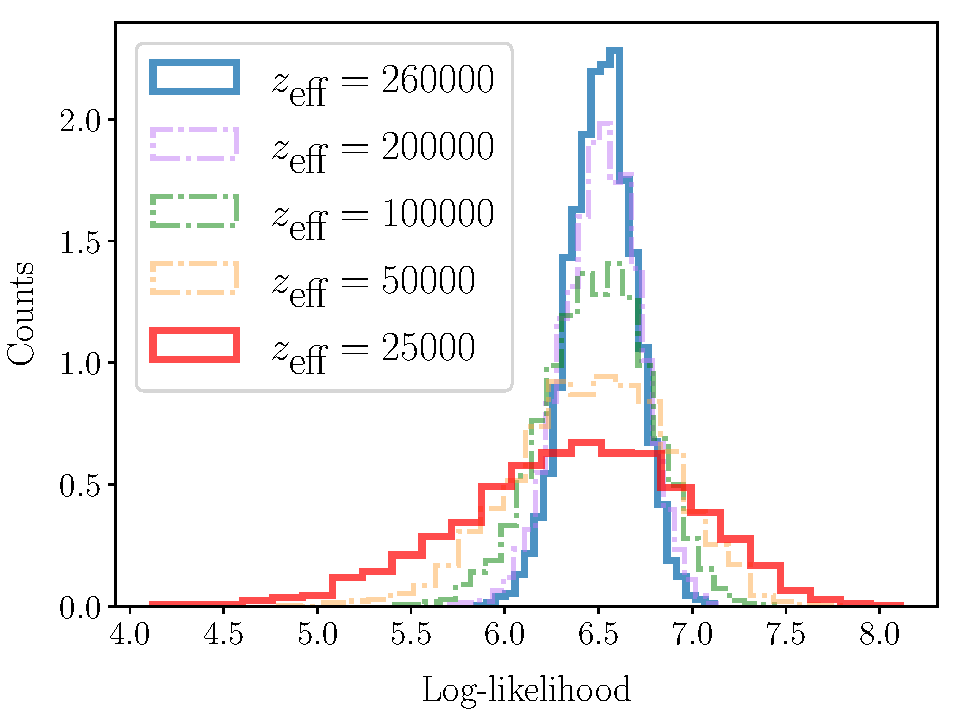
\includegraphics[width=.5\linewidth]{figs/hists_rect.pdf}
	\caption{Single sample log-likelihood error profiles for varying Monte Carlo batch sizes ($z_\textup{eff}$). We present the relationship between proposal log-likelihood reproducibility and $z_\textup{eff}$. Each profile represents a set of 5000 independent log-likelihood estimates for a single point in parameter space. Modelled as normal distributions, standard deviation decreases with increased $z_\textup{eff}$ (Eq.~\ref{eq:sigma}). The highlighted $z_\textup{eff}$ limits represent the batch sizes used for our 5000 and 100000 proposal posterior sample runs.}
	\label{fig:hists}
\end{figure}

\begin{align}\label{eq:sigma}
\sigma \propto \frac{1}{\sqrt{z_\textup{eff}}},
\end{align}

as expected from basic statistics of independent samples, where $\sigma$ is the standard deviation of the normal distribution fitted to the error profile. The reasoning behind the upper-limit on $z_\textup{eff}$ in Fig.~\ref{fig:hists} was previously explained in Section~\ref{method:monte} as being due to a combination of hardware and software limitations. However, the lower-limit of $z_\textup{eff}=25000$ is also linked to a software limitation of \texttt{tf.1}. When evaluating the decoder network at a location in the tails of the proposal posterior (a red sample in Fig.~\ref{fig:self_consist}), \texttt{tf.1} sets a hard minimum limit on this value, preventing meaningful analysis of lower log-likelihood values by truncating the density profile into a minimum bin. This binning of lower log-likelihoods is more pronounced for low $z_\textup{eff}$, causing any $z_\textup{eff}<25000$ error profile (as in Fig.~\ref{fig:hists}) to be severely negatively-skewed towards this lower-limit. Whilst this binning is still present in higher $z_\textup{eff}$, it is outweighed by the density of higher log-likelihood estimates. This binning prevents a more quantitative error analysis as, in its absence, we could estimate the error from Fig.~\ref{fig:hists} as $\sigma/\sqrt{5000}$. We could then determine the $z_\textup{eff}$ required to produce a proposal log-likelihood error of $\pm0.1$ to align with \texttt{Bilby} benchmark standards, providing a quantitative upper-limit on proposal reproducibility. This upper-limit forms one component of scatter in the data comparing proposal and target log-likelihoods. The second component of scatter originates from the discrepancy between proposal and target posteriors.

\begin{figure}
	\subfigure[Scatter profile of two independent proposal runs]{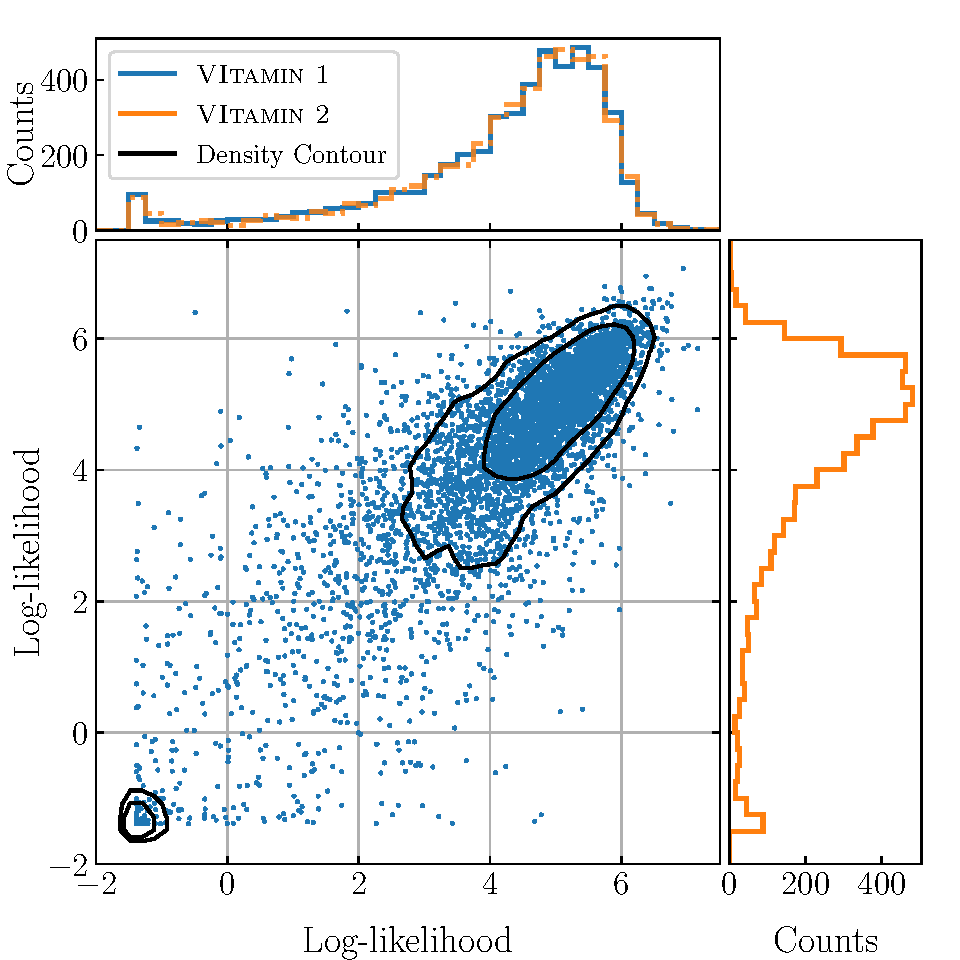
\includegraphics[width=.5\linewidth]{figs/vvscatter.pdf}}
	\subfigure[Scatter profile of target and proposal runs]{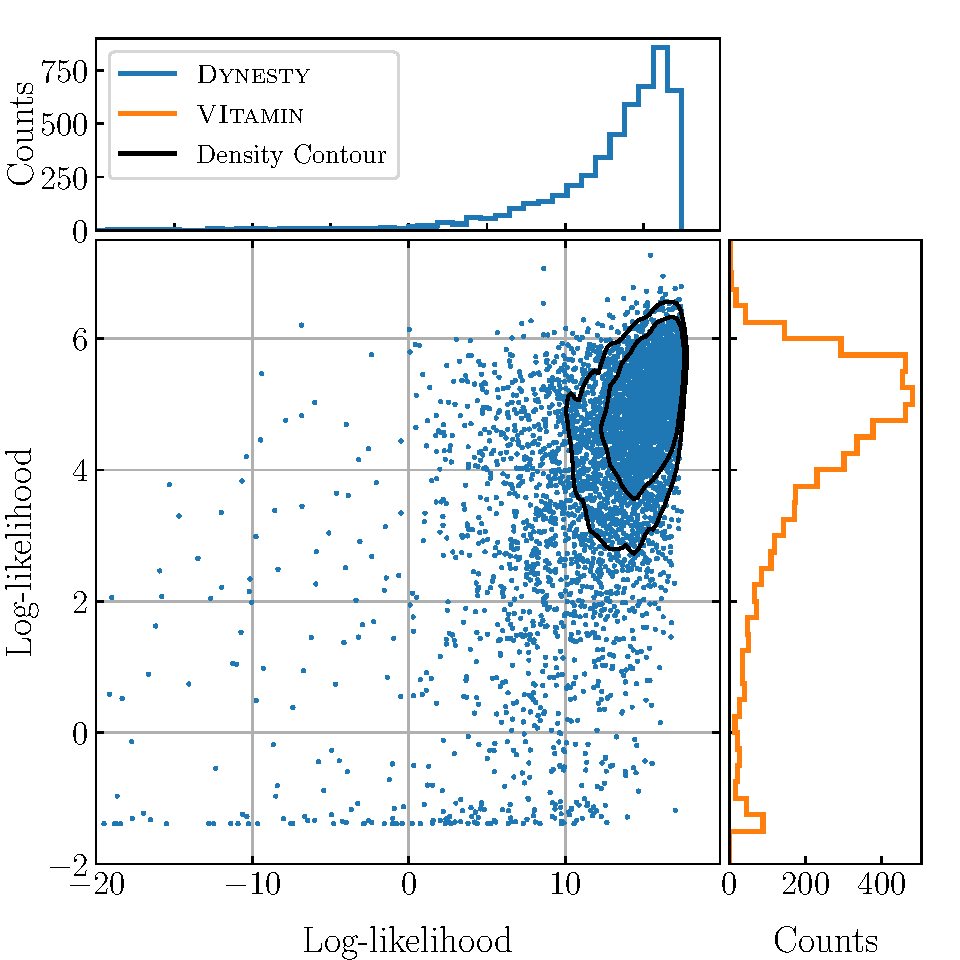
\includegraphics[width=.5\linewidth]{figs/bvscatter.pdf}}
	\caption{Scatter plots and profiles of independent log-likelihood runs. For our set of 5000 proposal posterior samples we ran two independent proposal log-likelihood estimates and one target log-likelihood estimate. Density contours (black) indicate the 50\% and 68\% confidence intervals of the scatters. Proposal runs truncate at low log-likelihood values whereas the target run log-likelihoods decrease naturally into the tails of distribution which accounts for inconsistent log-likelihood ranges between run methods.}
	\label{fig:scatter}
\end{figure}

Further analysis is done in Fig.~\ref{fig:scatter}(a) which presents the scatter in data of two independent proposal log-likelihood runs on the set of 5000 proposal posterior samples at $z_\textup{eff} = 260000$. By keeping the posterior consistent between both runs, we isolate the reproducibility scatter. The binning is identified in the top plot, as the tightly correlated profiles of both proposal runs truncate at the same lower limit, despite maximising $z_\textup{eff}$. These two runs are then presented as a scatter plot with a density contour of the 50\% and 68\% (1-$\sigma$) credible intervals plotted in black. For comparison, a perfectly deterministic approach would result in all scatter points lying on a line of unit gradient. Although fairly symmetrical about this line, the density contours show the detrimental effect of this binning, with a high density of low log-likelihoods flattened to the same minimum value. Figure~\ref{fig:scatter}(b) visualises the resultant of both sources of data scatter by comparing independent runs on proposal and target posteriors. The top plot shows the target log-likelihood profile with no evidence of binning as log-likelihood evaluations continue far into the natural tails of the distribution. The inconsistent truncation between runs skews the resultant scatter plot which loses its symmetry about the line of unit gradient, with a hard lower-limit in the proposal axis. These plots demonstrate the limitations on further analysis from software binning, which need to be addressed before a more quantitative measure of proposal reproducibility can be implemented. 



\subsection{Importance Resampling}\label{results:resample} %%%%%%%%%%%%%%%%%

\begin{figure}
	\centering
	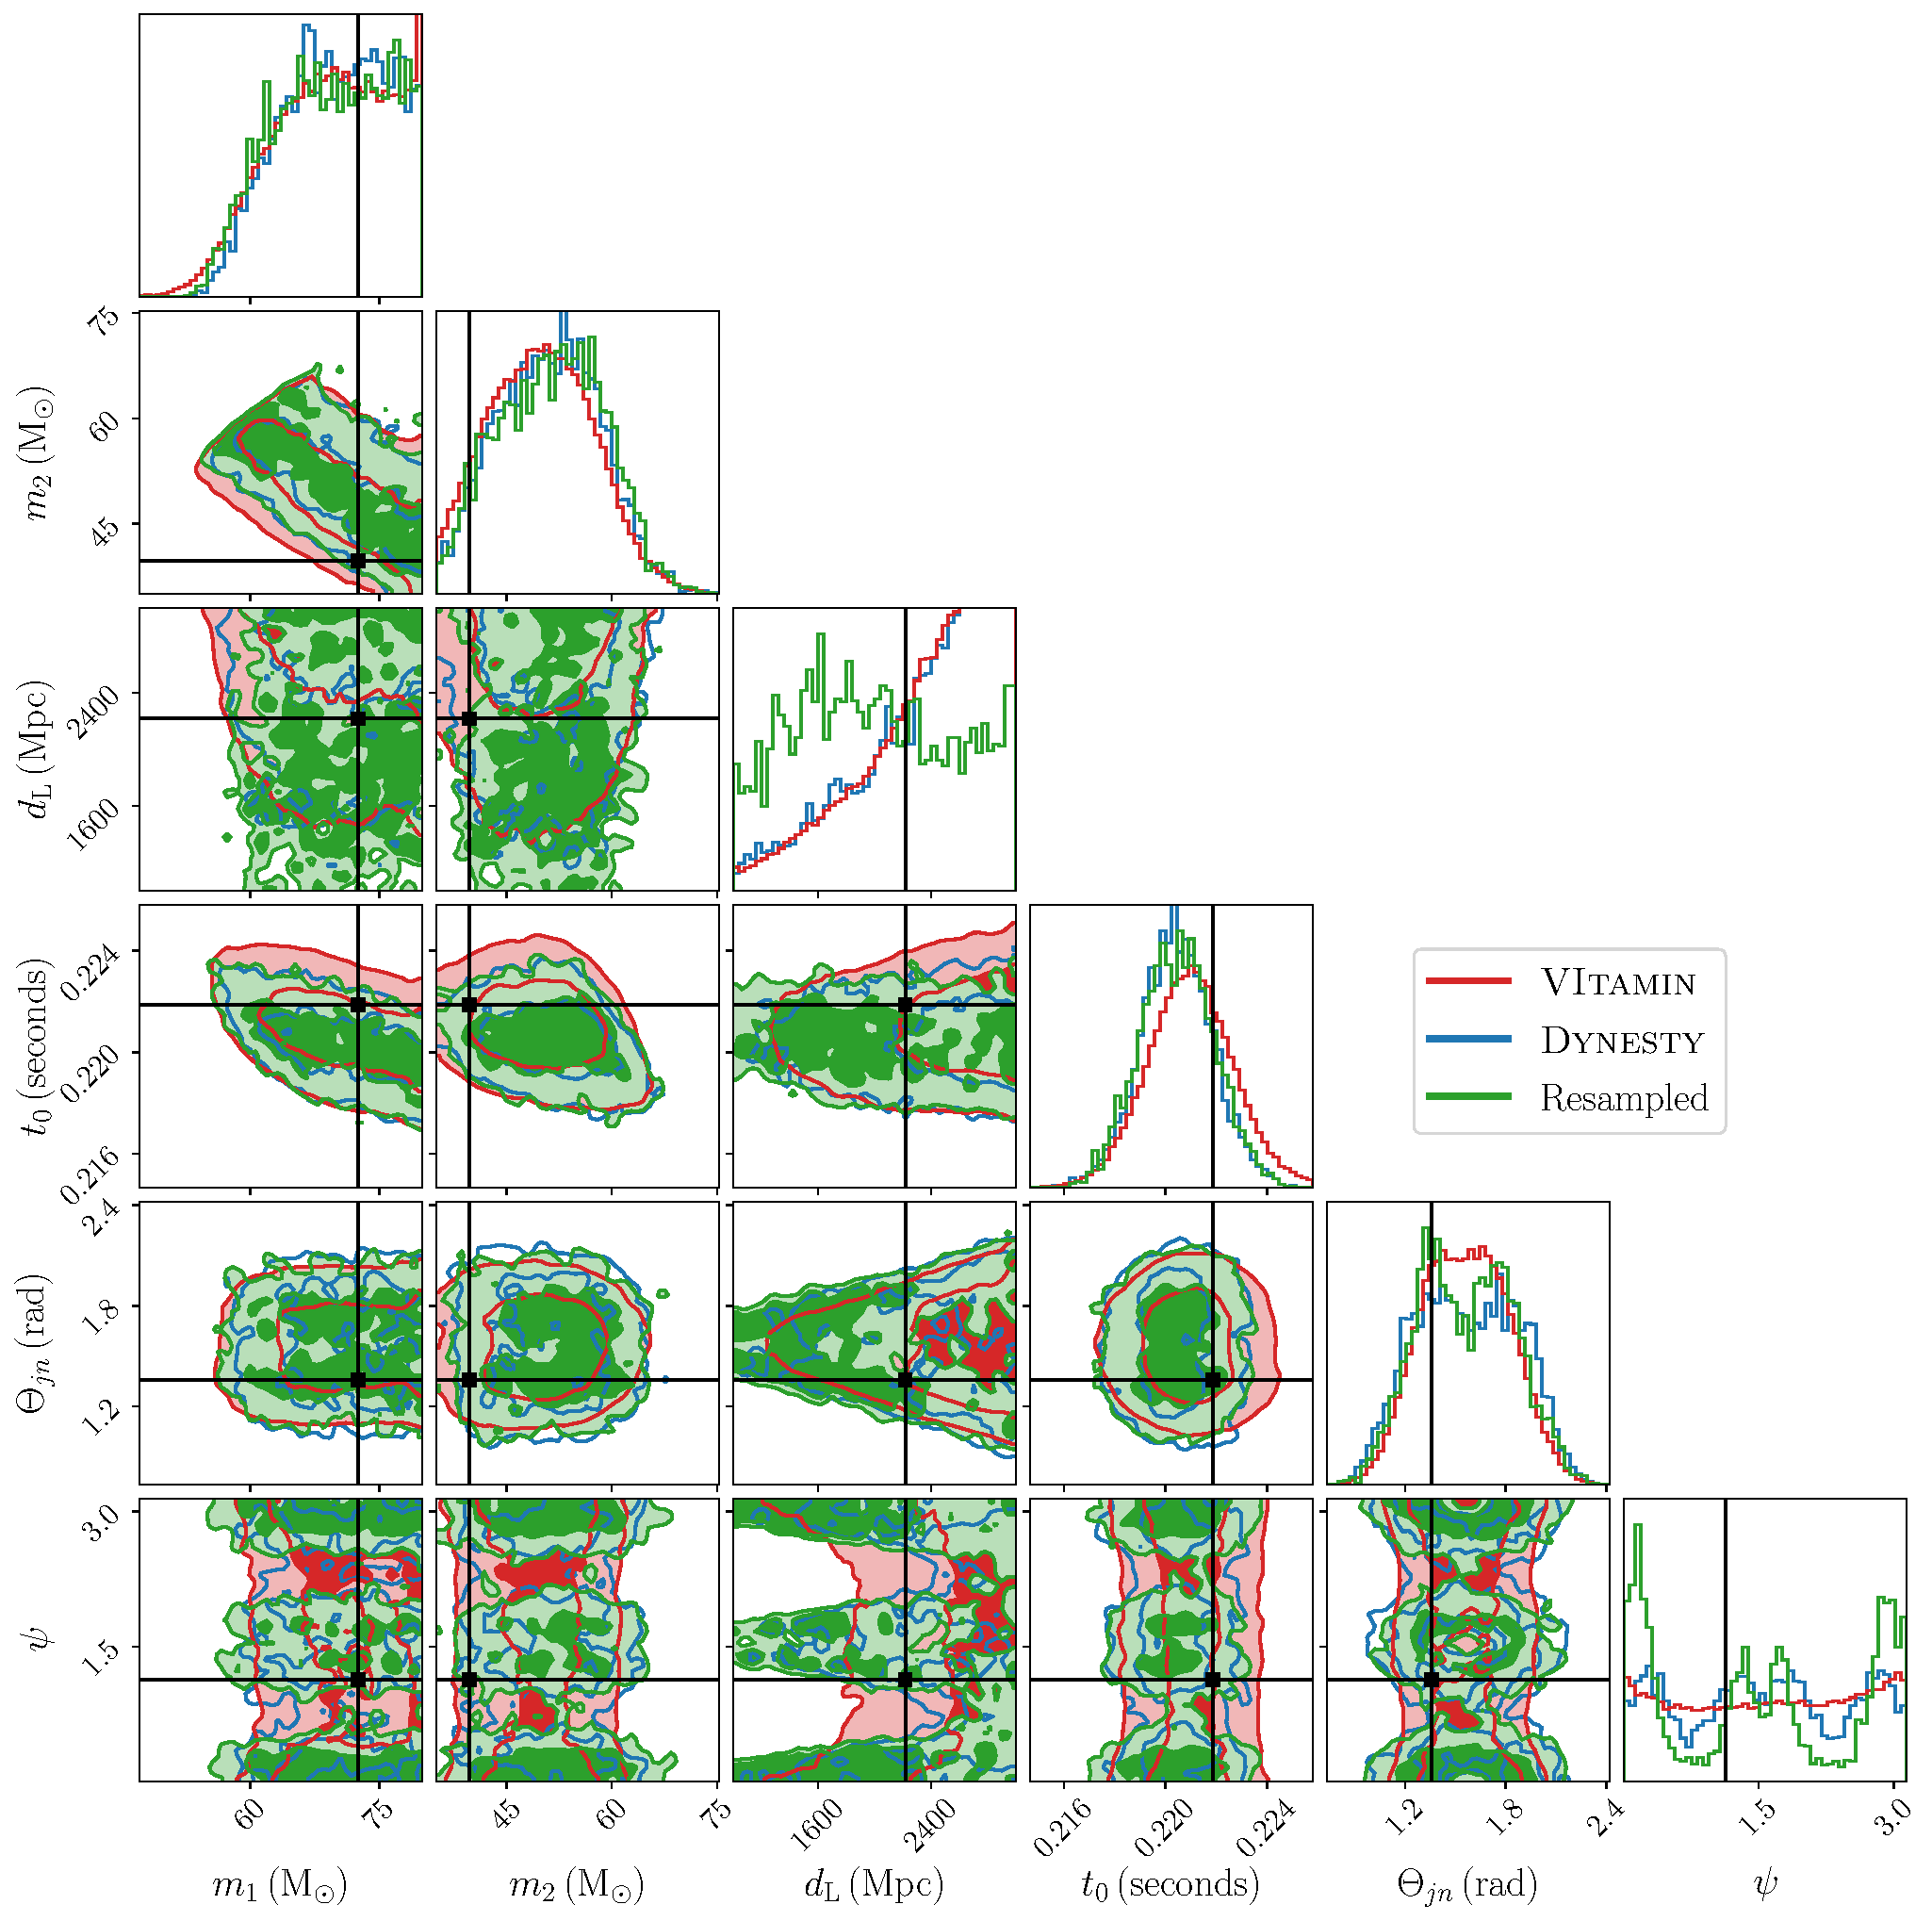
\includegraphics[width=\linewidth]{figs/resample_corner.pdf}
	\caption{Full corner plot comparing the 100000 sample proposal (red), 10000 sample target (blue) and 5000 sample resampled (green) posterior distributions for the 6 inferred parameters. True parameter values are shown in black and contours represent the 50\% and 90\% confidence intervals in the 2D distributions. Resampled posteriors show better sampling from multi-modal parameters compared with proposal with every 2D distribution showing resampled to be better aligned with target. Resampled distance posterior is, however, uninformative despite original proposal being well-fitted. }
	\label{fig:final_corner}
\end{figure}

Having carried out likelihood reweighting on our 100000 proposal samples with $z_\textup{eff}=25000$ in accordance with the methodology set out in Section~\ref{method:reweighting}, we present our findings in Fig.~\ref{fig:final_corner}. We start with the same data as in Fig.~\ref{fig:vit_train_corner} and overlay our resampled posterior in green. The first notable improvement is that the resampled posterior converges much better with the target posterior for the multi-modal parameters, where the proposal posterior is under-sampled. Looking at the 2D contours, the resampled posterior matches better with the target posterior in every case. In the 1D remit, all but distance show improvement, where the resampled distance posterior is very different to the target despite the proposal posterior being a good match. In testing, it was found that this uninformative distance posterior could be recreated using a subset of proposal posterior samples according to the 500 lowest log-likelihood locations from Fig.~\ref{fig:self_consist}. From these findings, this distance discrepancy is likely a consequence of $z_\textup{eff}=25000$ limitations (Fig.~\ref{fig:hists}), rather than a methodological failure. As a proof-of-concept, Fig.~\ref{fig:final_corner} shows great potential for likelihood reweighting as, in general, the resampled posterior matches the target better than the proposal posterior.


\section{Conclusions}\label{conc} %%%%%%%%%%%%%%%%%%%%%%%%%%%

In this paper, we have discussed the recent focus on rapid PE in preparation for multi-messenger astronomy. We have shown this pursuit of speed to be a driving motivation for increased \ac{DL} implementations in PE pipelines and have commented on the suitability of deep generative models for GW inference. We introduced our CVAE model \texttt{VItamin} (as defined in paper 1~\cite{vitpaper}) which boasts an inference speed-up of more than 6 orders of magnitude (Table~\ref{tab:speed}) compared to traditional sampling algorithms by using VI to circumvent costly likelihood calculations. The trade-off between speed and versatility between VI and NS methods was discussed with an emphasis on the importance of being able to estimate likelihoods during inference to evaluate the Bayesian evidence (Eq.~\ref{eq:bayes_evidence}) and carry out useful auxiliary techniques, such as likelihood reweighting. We discussed the success of a recent paper~\cite{resample_aus} in using SIR methods to reweight the proposal posterior from an approximate waveform and highlighted the compatibility of their method with our likelihood reweighting task.

In Section 2, we created a \texttt{VItamin} model for our sub-parameter space. In Fig.~\ref{fig:vit_train_corner}, we presented the end state of this model's incomplete training phase as a benchmark proposal posterior $r_\theta(x|y)$ to improve upon, using our \texttt{dynesty} target $p(x|y)$. We then used Monte Carlo methods to estimate $r_\theta(x|y)$ at a single position in parameter space (Eq.~\ref{eq:monte_approx2}) and were able to equate this to a proposal likelihood, as a consequence our selective choice in parameters with flat priors (Eq.~\ref{eq:post_like}). We then described the SIR framework required to reweight our proposal samples using the proposal likelihood estimates, following the methodology of~\cite{resample_aus} and the fixed resample ratio of 20 suggested in~\cite{brian2006resampling}.

In Section 3, our proposal likelihoods passed their qualitative self-consistency test (Fig.~\ref{fig:self_consist}) which is a mandatory internal check needed before comparing with other algorithms. We showed that increasing the Monte Carlo batch size ($z_\textup{eff}$) increased the reproducibility of our method (Fig.~\ref{fig:hists}), but attempts at more quantitative error analysis were prevented by software limitations originating in the antiquated \texttt{tf.1} framework that \texttt{VItamin} was written in at the time of work. These software limitations were two-fold. First, an unavoidable memory leak placed an upper-limit on $z_\textup{eff}$, capping further efforts to suitably minimise error. Secondly, inherent binning of low likelihood values in the code made in-depth profile analyses of proposal likelihood runs impossible and limited the ability to compare values with the target method due to inconsistent truncation (Fig.~\ref{fig:scatter}). A priority of future work is to re-code our Monte Carlo algorithm (Fig.~\ref{fig:monte_flow}) in the updated \texttt{keras.tensorflow} framework of \texttt{VItamin} which we predict to fix both software limitations. Once fixed, a complete error analysis can be applied to our proposal method to derive the minimum $z_\textup{eff}$ required to produce a log-likelihood error of $\pm1$ which is comparable to the quoted tolerance in other sampling algorithms.

In Fig.~\ref{fig:final_corner}, we present our final reweighted results which align better with our target posterior, as desired. This plot shows the specific capabilities of resampling to improve multi-modal posteriors, whose topology was previously missed. The resampled distance posterior became uninformative but we were able to replicate this discrepancy in a fixed low log-likelihood framework. Considering that these log-likelihoods were capped at $z_\textup{eff}=25000$, due to the aforementioned software limitations, we are confident that these results successfully show the significant potential of Monte Carlo methods in increasing the versatility of DL for GW inference.

Taking these findings from proof-of-concept to production status requires a significant overhaul in methodology and flexibility. Firstly, we need to expand our posterior dimension to encompass the entire 15 parameter space. This means working with non-flat priors, and so requiring a more involved approach than Eq.~\ref{eq:post_like} in converting from proposal posterior to likelihood. Secondly, the resampling speed must be dramatically increased to be useful in rapid PE, as computing our 100000 proposal likelihoods required a run-time of 6 hours. A straightforward first step towards this is to decrease the number of original proposal posterior samples from 100000. However, if we desire a meaningful number of reweighted samples, we must update our primitive fixed sampling ratio approach. An improved SIR framework is presented in~\cite{10.2307/4616798} that claims to significantly reduce the required sampling ratio by minimising resampling bias. Expanding the parameter space and reducing computing time, lend themselves to be the intuitive next steps in this process, with potential for this method to help accelerate the practical realisation of multi-messenger astronomy. 


\section*{Acknowledgements}


I would like to thank my supervisor Chris Messenger for his support and guidance throughout this project. I would also like to thank Hunter Gabbard for his insight and patience explaining and modifying \texttt{VItamin} for my use case. I am also indebted to Michael Williams and Daniel Williams for their continued technical support. Finally, I would like to express my gratitude toward the entire University of Glasgow IGR-data analysis group for making me feel very welcome over the past year.

% \break
\printbibliography[
heading=bibintoc,
title={References}
]

\end{document}



